\documentclass[11pt]{article}
\usepackage{geometry} % See geometry.pdf to learn the layout options. There are lots.
\geometry{letterpaper} % ... or a4paper or a5paper or ...
%\geometry{landscape} % Activate for for rotated page geometry
%\usepackage[parfill]{parskip} % Activate to begin paragraphs with an empty line rather than an indent
\usepackage{graphicx}
\usepackage{amssymb}
\usepackage{epstopdf}
\usepackage{listings}
\usepackage[usenames,dvipsnames]{color}
\definecolor{lightgray}{rgb}{0.9,0.9,0.9}
\definecolor{darkgray}{rgb}{0.5,0.5,0.5}
\lstloadlanguages{R} 



\DeclareGraphicsRule{.tif}{png}{.png}{`convert #1 `dirname #1`/`basename #1 .tif`.png}

\title{Assignment 3}
\author{The Author}
\date{} % Activate to display a given date or no date

\begin{document}
\maketitle
\lstset{% general command to set parameter(s)
language=R,
basicstyle=\scriptsize \ttfamily,
commentstyle=\ttfamily \color{darkgray},
numbers=left,
numberstyle=\ttfamily \color{darkgray} \footnotesize,
stepnumber=1,
numbersep=5pt,
backgroundcolor=\color{lightgray},
showspaces=false,
showstringspaces=false,
showtabs=false,
frame=single,
tabsize=2,
captionpos=b,
breaklines=true,
breakatwhitespace=false,
title=\lstname,
escapeinside={},
keywordstyle={},
morekeywords={}}


\section{Neural Networks}
\subsection{Derivation of the derivative of the transfer function}

The transfer function is given by the equation $ \sigma(u) = \frac{u}{1+|u|}$. We define $f(u)=u$ and $g(u)=1+|u|$, where via the quotient rule $\sigma'(u)=\frac{f'(u)g(u)-f(u)g'(u)}{g(u)^2}$
\[
\sigma'(u)=\frac{(|u|+1)  (\frac{d}{du}(u)) - u(\frac{d}{du}(|u|+1))
}
{(|u|+1)^2
}
=\frac{ -u(\frac{d}{du}(|u|+1)) +|u| +1 }
{(|u|+1)^2} =
\]
\[
=\frac{ -u(\frac{d}{du}(|u|)) +|u| + 1}
{(|u|+1)^2}
\]
Given that $\frac{d}{du}|u|=\frac{u}{|u|}$, $\frac{d}{du}|u|=1$ if $u>0$ and $\frac{d}{du}|u|=-1$ if $u<0$, so $-u(\frac{d}{du}(|u|+1))=0$ for every value of $u$, which leads us to:
\[
 \sigma(u) = \frac{1}{(1+|u|)^2} \blacksquare
\]

We implemented a neural network using one hidden layer and bias variables for the input layer and hidden layer. An illustration is shown below in figure \ref{graph}.


\begin{figure}[h!]
  \centering
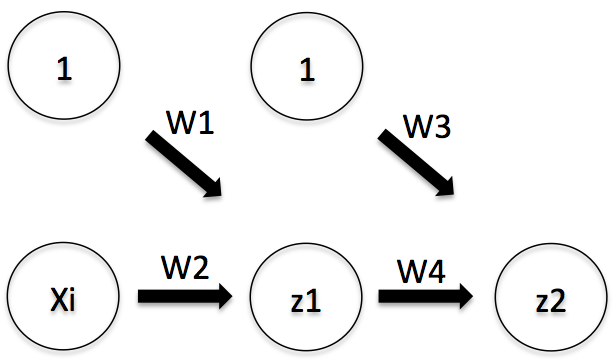
\includegraphics[width=0.4\textwidth]{graph.png}
\caption{A simple neural network. Nodes with 1 use for biases}
\label{graph}
\end{figure}

We do forward propagation on all 50 observations on which basis we calculate both layers of deltas. The deltas are then used to compute the analytical estimates for the sensitivity of the error function wrt a marginal change in each weight. The table below shows the calculated analytical estimates. Columns 2-5 represent weights w1,\ldots, w4 as illustrated in the figure above.


\begin{lstlisting}
[1,] -3.944795e-02 -2.346801e-01 -2.773737e-08 -1.620305e-08
[2,]  1.323323e-01 -1.371757e-01 -3.506232e-09  2.874986e-10
[3,] -1.308633e-01 -4.261930e-01 -2.155317e-08 -1.525527e-08
[4,]  4.594561e-03  3.595024e-02 -1.794995e-08  4.864099e-09
[5,] -7.245971e-02  2.612904e-01 -6.685206e-09  1.864244e-09
[6,] -1.378980e-01 -4.296404e-01 -1.019282e-08  4.650537e-09
[7,]  3.821643e-04 -2.975905e-03 -4.892959e-09 -1.469790e-09
[8,] -8.640731e-04  6.565295e-03 -5.191691e-09 -1.164102e-09
[9,] -7.820110e-02 -1.629617e-01 -6.423751e-09 -8.986778e-10
[10,] -1.134140e-01 -4.517279e-01  4.193329e-09  2.241183e-09
[11,]  8.574312e-03  6.911000e-02 -1.945228e-09 -4.057307e-09
[12,]  5.800364e-03  4.570548e-02  1.264099e-09  8.758006e-09
[13,] -3.580888e-02  8.797060e-02 -5.608467e-09 -9.493721e-11
[14,]  7.950451e-03 -1.711510e-02 -4.872648e-09 -2.004354e-10
[15,] -1.155483e-01 -4.011780e-01  2.321246e-09 -8.173090e-09
[16,] -1.244641e-01 -4.440829e-01  2.141503e-09  5.690569e-09
[17,] -7.228444e-02  3.059532e-01 -7.951222e-09  3.027517e-10
[18,] -1.445235e-02 -9.873281e-02 -3.047693e-10 -6.757340e-09
[19,]  1.764088e-03 -1.673568e-02 -5.591665e-09 -1.788593e-09
[20,]  1.906040e-02  1.656793e-01 -1.923726e-08  2.916423e-09
[21,]  6.223847e-02 -9.658540e-02 -4.221869e-09 -2.563358e-10
[22,]  5.888236e-02  5.401308e-02 -4.182799e-09 -5.019964e-10
[23,] -9.228407e-02 -4.309186e-01  3.081297e-09  1.193331e-08
[24,] -2.003189e-03  1.554559e-02 -5.513153e-09 -1.018322e-09
[25,] -1.229681e-01 -3.486650e-01 -1.105464e-08 -3.015099e-09
[26,] -1.685241e-02 -1.123710e-01 -1.194025e-08 -6.875160e-09
[27,]  3.544795e-02  3.399905e-01 -2.520039e-09  5.689736e-09
[28,] -4.538215e-04  3.769979e-03 -5.407649e-09 -1.071574e-09
[29,] -4.102944e-04  3.240866e-03 -5.144585e-09 -1.396538e-09
[30,] -9.263113e-02 -4.209148e-01 -2.031498e-08 -2.251438e-08
[31,] -8.626814e-03  1.684928e-02 -5.121230e-09 -2.401376e-10
[32,] -3.589918e-03  2.567554e-02 -5.539222e-09 -1.164118e-09
[33,] -4.906134e-02 -2.790409e-01  7.667397e-09 -8.028284e-09
[34,] -6.253433e-02 -3.322893e-01 -1.629686e-08  5.238479e-09
[35,] -3.638030e-02  1.999923e-01 -6.911953e-09 -5.067088e-11
[36,]  2.095151e-01 -1.262861e-01 -2.859786e-09 -3.710515e-09
[37,] -6.487128e-02 -3.425969e-01  1.115150e-09  1.764046e-08
[38,] -8.545768e-02  3.412778e-01 -5.361873e-09  2.052032e-09
[39,]  1.609653e-04 -1.362865e-03 -4.642265e-09 -2.021025e-09
[40,] -2.977619e-02  6.788642e-02 -5.431229e-09 -1.319273e-10
[41,] -6.801526e-02  3.082179e-01 -5.364083e-09  7.604643e-10
[42,] -1.533508e-02 -1.026128e-01  1.437487e-09  6.551818e-09
[43,] -3.589323e-02 -2.157753e-01 -9.017474e-09 -1.077246e-08
[44,]  8.378927e-02 -1.272164e-01 -3.953102e-09 -6.087516e-10
[45,]  1.312527e-01  5.011873e-02 -3.435255e-09  1.929682e-09
[46,] -8.984398e-02  3.321424e-01 -7.077325e-09 -3.801977e-10
[47,]  1.015527e-03 -9.102182e-03 -5.661946e-09 -1.519805e-09
[48,] -7.399453e-05  5.891379e-04 -5.028076e-09 -1.430685e-09
[49,] -1.046974e-02  6.732186e-02 -6.016270e-09 -2.719607e-10
[50,]  3.651611e-10 -1.110040e-08 -5.487058e-09 -1.367696e-09
\end{lstlisting}
While estimates could be computed using the numerical estimates, this procedure is computationally expensive. For that reason we only use them for valiation of the analytical estimates. 

Our implementation is attached in the file \texttt{3.1.1.R}.

\subsection{Neural Network Training}
Our implementation of a neural network with an arbitrary number of neurons in a single layer, is found in the file \texttt{3.1.2.R}. Despite not using early stopping or regularization of any sort, we did not observe any over-fitting, as demonstrated by figure \ref{goodplot}. This can be ascribed to the model --- using 20 neurons --- not being complicated enough to over fit the data. To avoid overfitting on a more complicated model we would use early stopping; that is, divide our dataset into a training and testing subset, and then look at the error of the test dataset, and stop training when the error begins increasing. 

\begin{figure}[h!]
  \centering
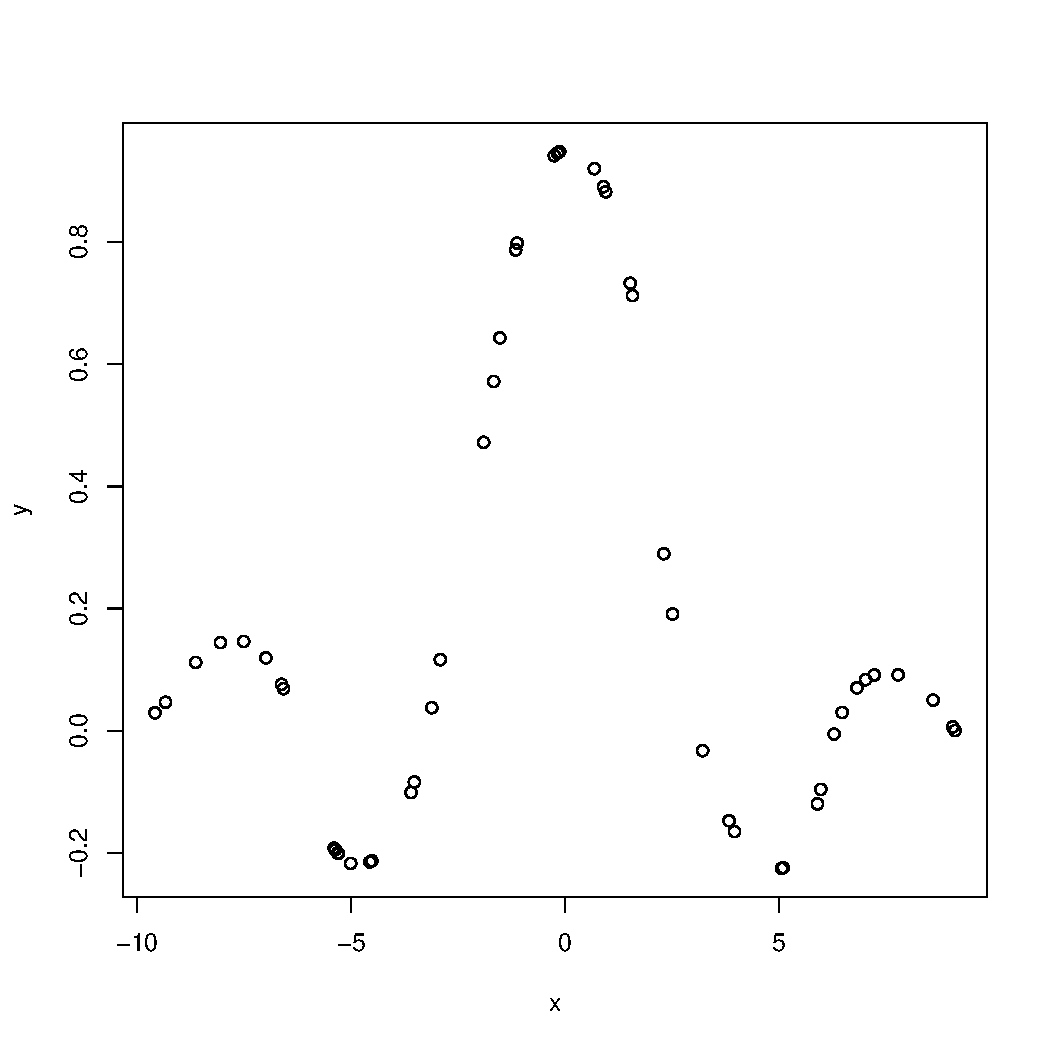
\includegraphics[width=0.45\textwidth]{out-001-10000-20.pdf}
\caption{Using 20 neurons, 10000 iterations, and a learning rate of 0.01, neural networks learn the underlying distribution. Further, we see no evidence of overfitting, despite not using early stopping}
\label{goodplot}
\end{figure}



\section{Support Vector Machines}
\subsection{Model Selection Using Grid Search}
We train our support vector machine using the \texttt{ksvm} function found in the \texttt{kernlab R} module. An example of the syntax is as follows:
\begin{lstlisting}
ksvm(V3~.,data=kc200,kernel='rbfdot',cross=5,C=C[j],kpar=list(sigma=sigma[i]))
\end{lstlisting}
We use the `formula' notation, which takes the form \texttt{targetVariable\textasciitilde features}. N-fold cross validation is performed by setting the \texttt{cross} parameter to N. The function automatically splits the dataset into N parts, trains the model on the first N-1 parts and tests on the last part, then takes another N-1 parts, etc, N times in total, after which it returns the average error of the N models it has trained and tested. The kernel used is specified by the \texttt{kernel} parameter, and \texttt{rbfdot} is a gaussian kernel. The kernel's parameters are set by passing list to the \texttt{kpar} parameter, and the gaussian kernel has a single parameter, $\sigma$. The \texttt{C} parameter of the SVM is set by using the \texttt{C} parameter in the function.

In order to determine the optimal \texttt{C} and $\sigma$ parameters, we use a grid search: we test reasonable combinations of $\sigma$ and \texttt{C}, and then choose the parameters which have the lowest cross-validation error. After looking at seven different $\gamma$ and $C$ parameters, for the dataset with 400 observations, we get the following error rates using 5-fold cross validation:\\
\begin{tabular}{|c|c|c|c|c|c|c|c|}
\hline
C,$\gamma$&1e-05 & 0.01 & 0.05 & 1 & 3 & 7 & 10000\\\hline
0.1&0.5750&0.0325&0.0275&0.0250&0.0250&0.0250&0.3925\\\hline
1 & 0.1725 & 0.0325 & 0.0300 & 0.0250&0.0275&0.0275&0.0275\\\hline
10&0.1950&0.0375&0.0375&0.0300&0.0250&0.0250&0.0250\\\hline
100&0.2275&0.0375&0.0400&0.0275&0.0250&0.0250&0.0275\\\hline
1000&0.1975&0.0375&0.0400&0.0375&0.0450&0.0325&0.0250\\\hline
10000&0.2225&0.0725&0.0550&0.0325&0.0350&0.0425&0.0275\\\hline
\end{tabular}

For the dataset with 200 observations, we get the following errors:\\
\begin{tabular}{|c|c|c|c|c|c|c|c|}
\hline
C,$\gamma$ &1e-05&0.01&0.05&1&3&7&10000\\\hline
0.1&0.560&0.065&0.040&0.030&0.020&0.015&0.485\\\hline
1&0.375&0.040&0.040&0.030&0.025&0.020&0.025\\\hline
10&0.320&0.050&0.040&0.020&0.035&0.030&0.015\\\hline
100&0.315&0.045&0.035&0.040&0.015&0.035&0.030\\\hline
1000&0.315&0.060&0.035&0.030&0.035&0.030&0.020\\\hline
10000&0.345&0.045&0.030&0.045&0.045&0.035&0.020\\\hline
\end{tabular}

For the dataset with 100 observations, we get the following errors:\\
\begin{tabular}{|c|c|c|c|c|c|c|c|}
\hline
C,$\gamma$& 1e-05 & 0.01 & 0.05 & 1 & 3 & 7 & 10000\\\hline
0.1 & 0.53 & 0.44 & 0.07 & 0.04 & 0.02 & 0.03 & 0.44\\\hline
1 & 0.34 & 0.03 & 0.05 & 0.02 & 0.03 & 0.03 & 0.02\\\hline
10 & 0.29 & 0.04 & 0.02 & 0.02 & 0.06 & 0.05 & 0.02\\\hline
100 & 0.42 & 0.03 & 0.08 & 0.03 & 0.05 & 0.03 & 0.02\\\hline
1000 & 0.34 & 0.05 & 0.04 & 0.03 & 0.02 & 0.04 & 0.02\\\hline
10000 & 0.39 & 0.02 & 0.05 & 0.04 & 0.04 & 0.03 & 0.03\\\hline
\end{tabular}

As such with pick the hyper parameters $(\gamma,C)=(1,1),(3,100),(1,1)$ for $N=400,200,100$ observations respectively.

The test errors for the dataset with 200 observations are as follows (we can see the model over fitting with small $C,\gamma$ parameters):\\
\begin{tabular}{|c|c|c|c|c|c|c|c|}
\hline
C,$\gamma$&1e-05 & 0.01 & 0.05 & 1 & 3 & 7 & 10000\\\hline
0.1 & 0 & 0.005 & 0.010 & 0.020 & 0.020 & 0.020 & 0.050\\\hline
1 & 0 & 0.005 & 0.010 & 0.015 & 0.020 & 0.025 & 0.020\\\hline
10 & 0 & 0.000 & 0.005 & 0.015 & 0.015 & 0.015 & 0.015\\\hline
100 & 0 & 0.000 & 0.000 & 0.015 & 0.015 & 0.015 & 0.015\\\hline
1000 & 0 & 0.000 & 0.000 & 0.000 & 0.010 & 0.015 & 0.015\\\hline
10000 & 0 & 0.000 & 0.000 & 0.000 & 0.000 & 0.000 & 0.015\\\hline
\end{tabular}
\subsection{Inspecting the Kernel Expansion}
\subsubsection{Visualizing the SVM solution}
\begin{figure}[h!]
  \centering
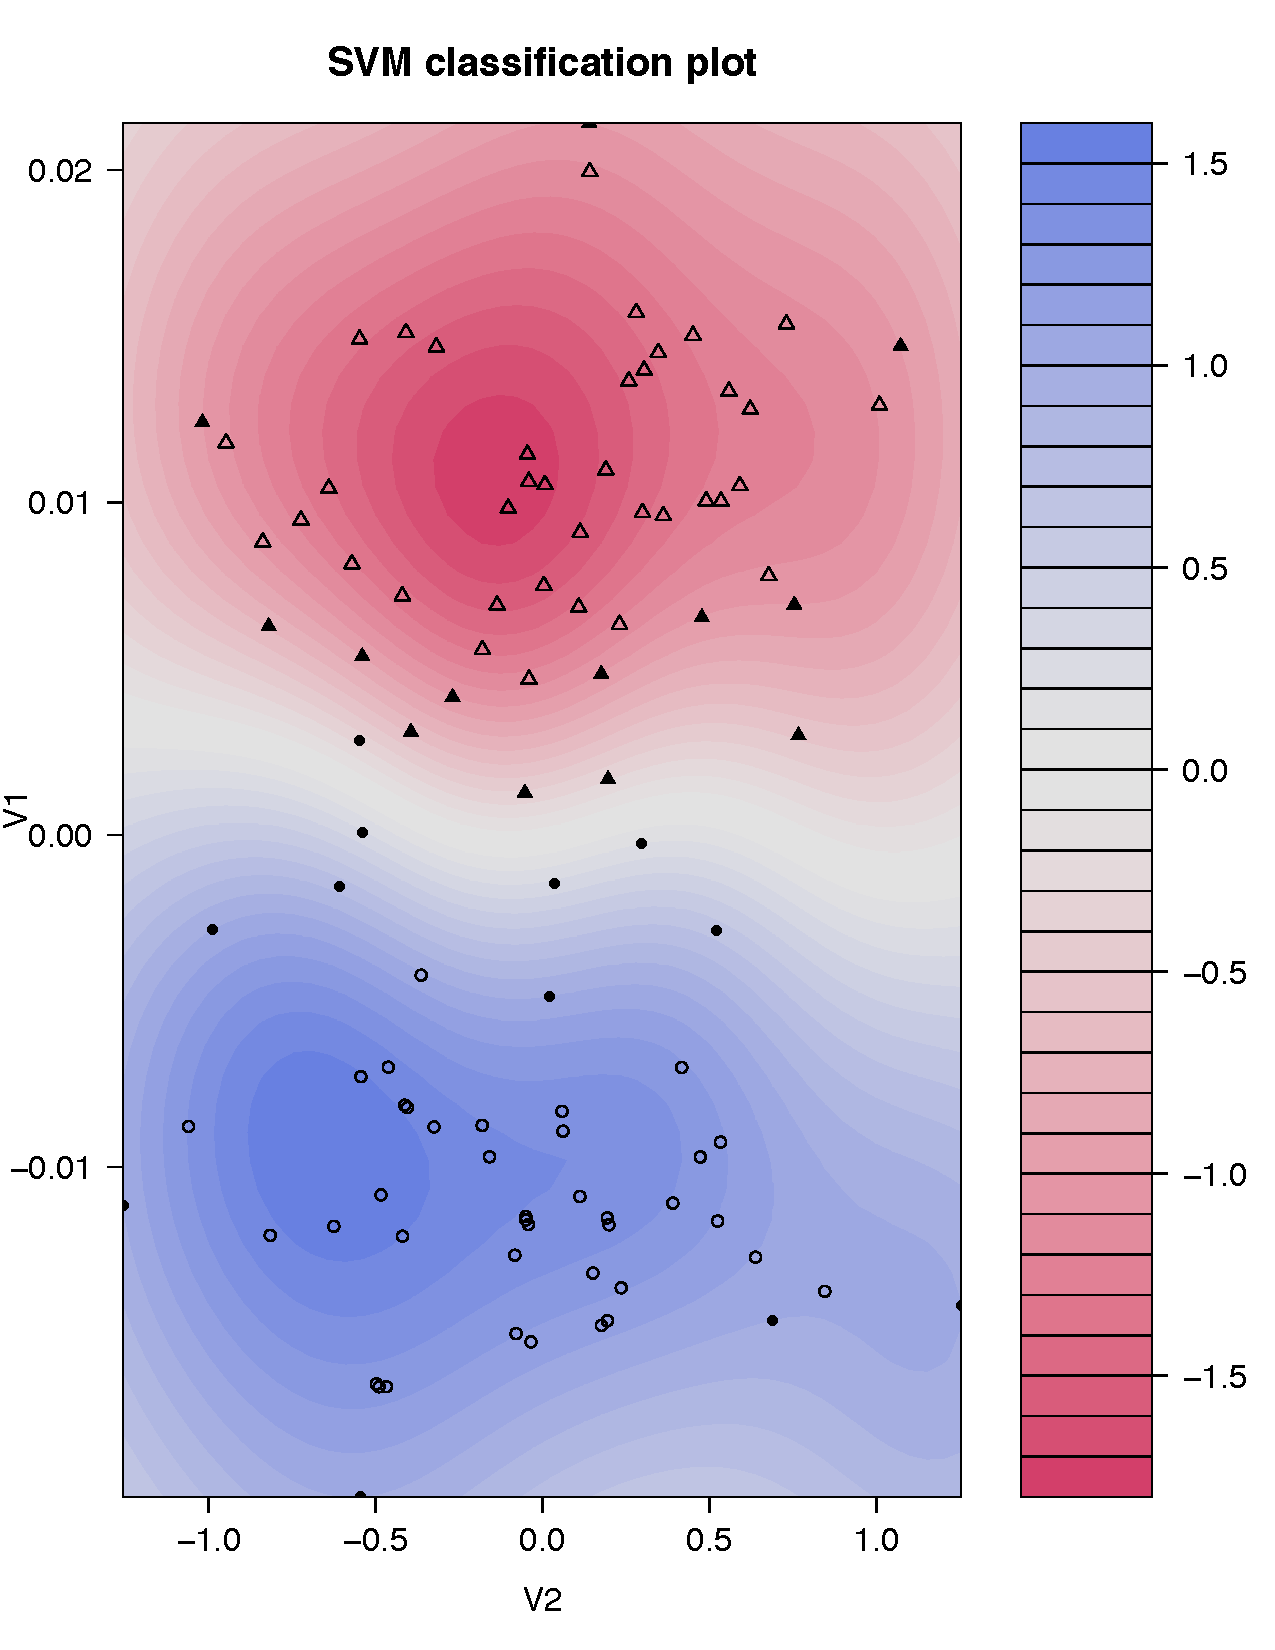
\includegraphics[width=0.5\textwidth]{2-2.pdf}
\caption{ Bound vectors represented in black. Unbound vectors are clear }
\label{bound}
\end{figure}
\subsubsection{Effect of the Regularization Parameter}
The regularization parameter C controls the trade-off between the maximization of the margin, and the number of errors performed on a test data set. In figure \ref{smallC} we show a plot with C=0.01 and figure \ref{bigC} shows a plot with C=100. Note the larger amount of bound vectors present when using the small value of C.
\begin{figure}[h!]
  \centering
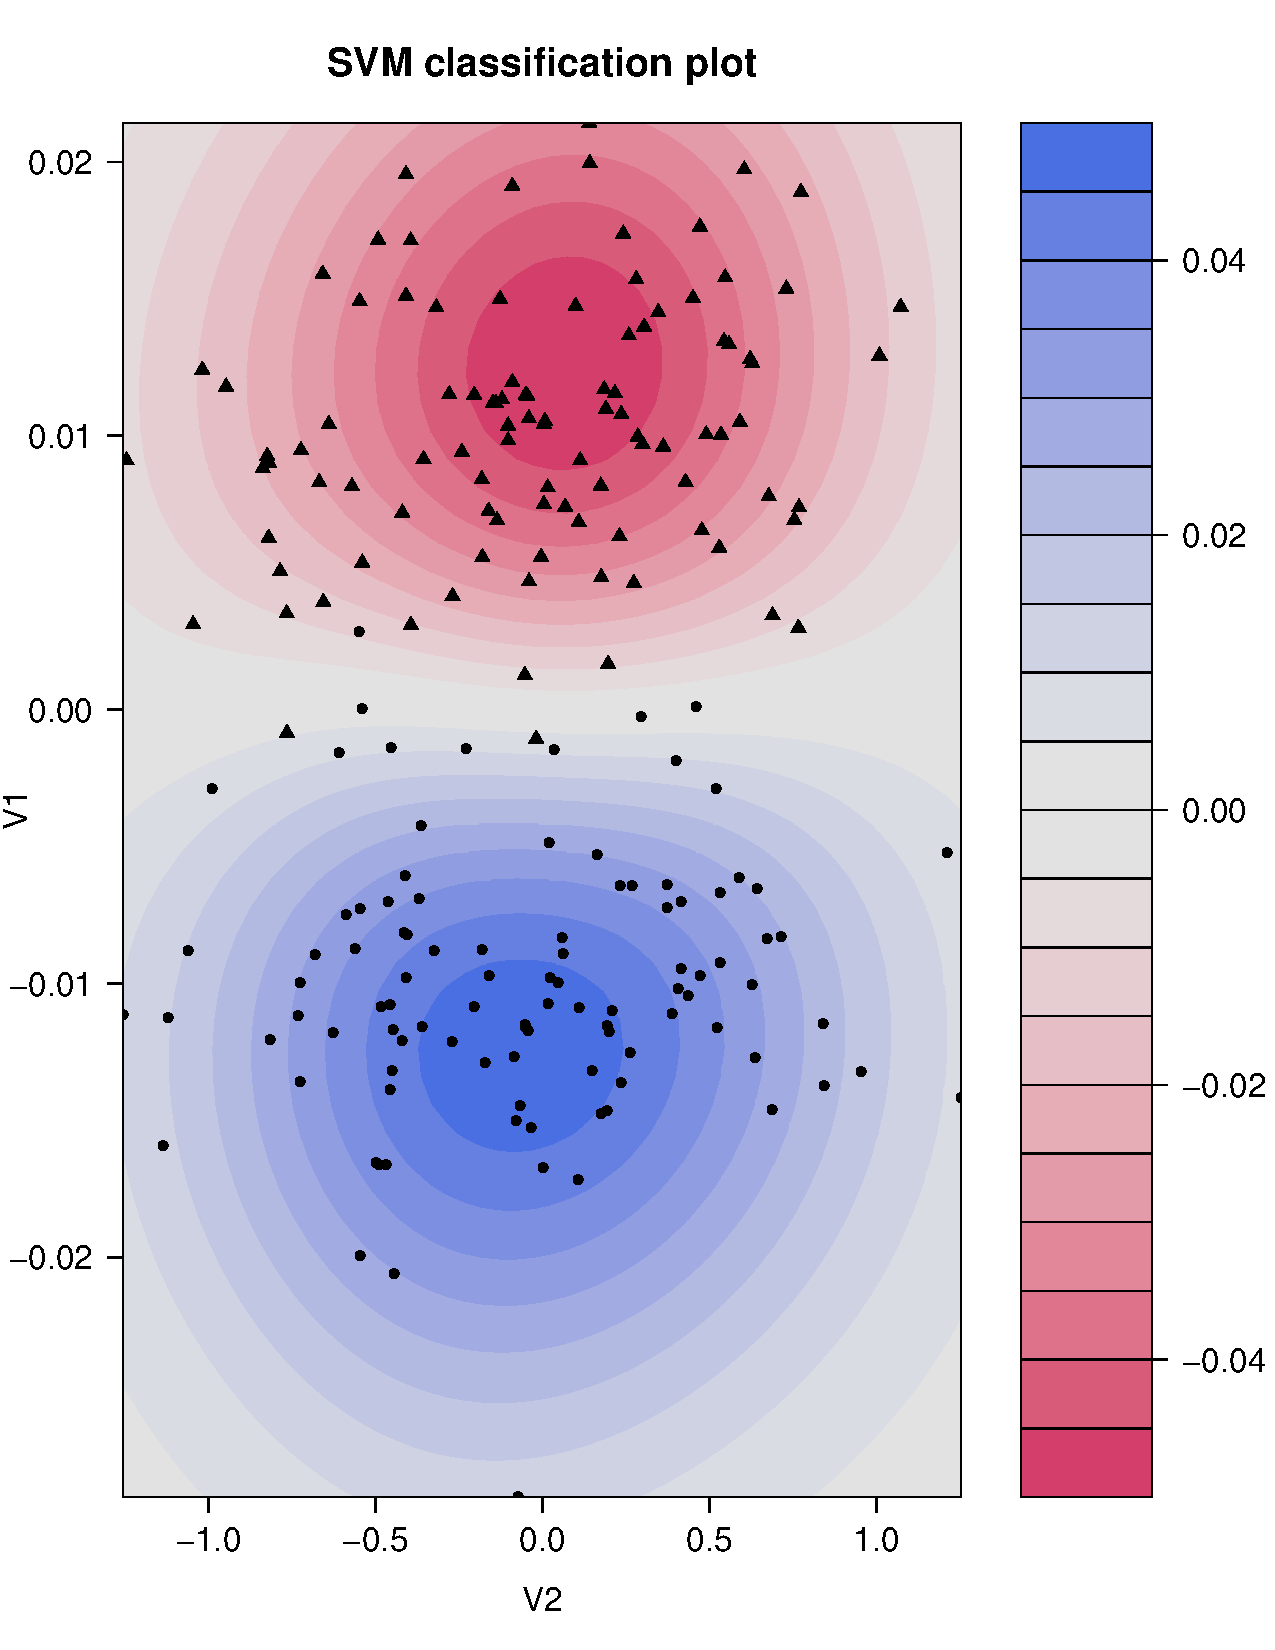
\includegraphics[width=0.5\textwidth]{smallC}
\caption{visualization with $\gamma=1$ and $C=0.001$ }
\label{smallC}
\end{figure}
\begin{figure}[h!]
  \centering
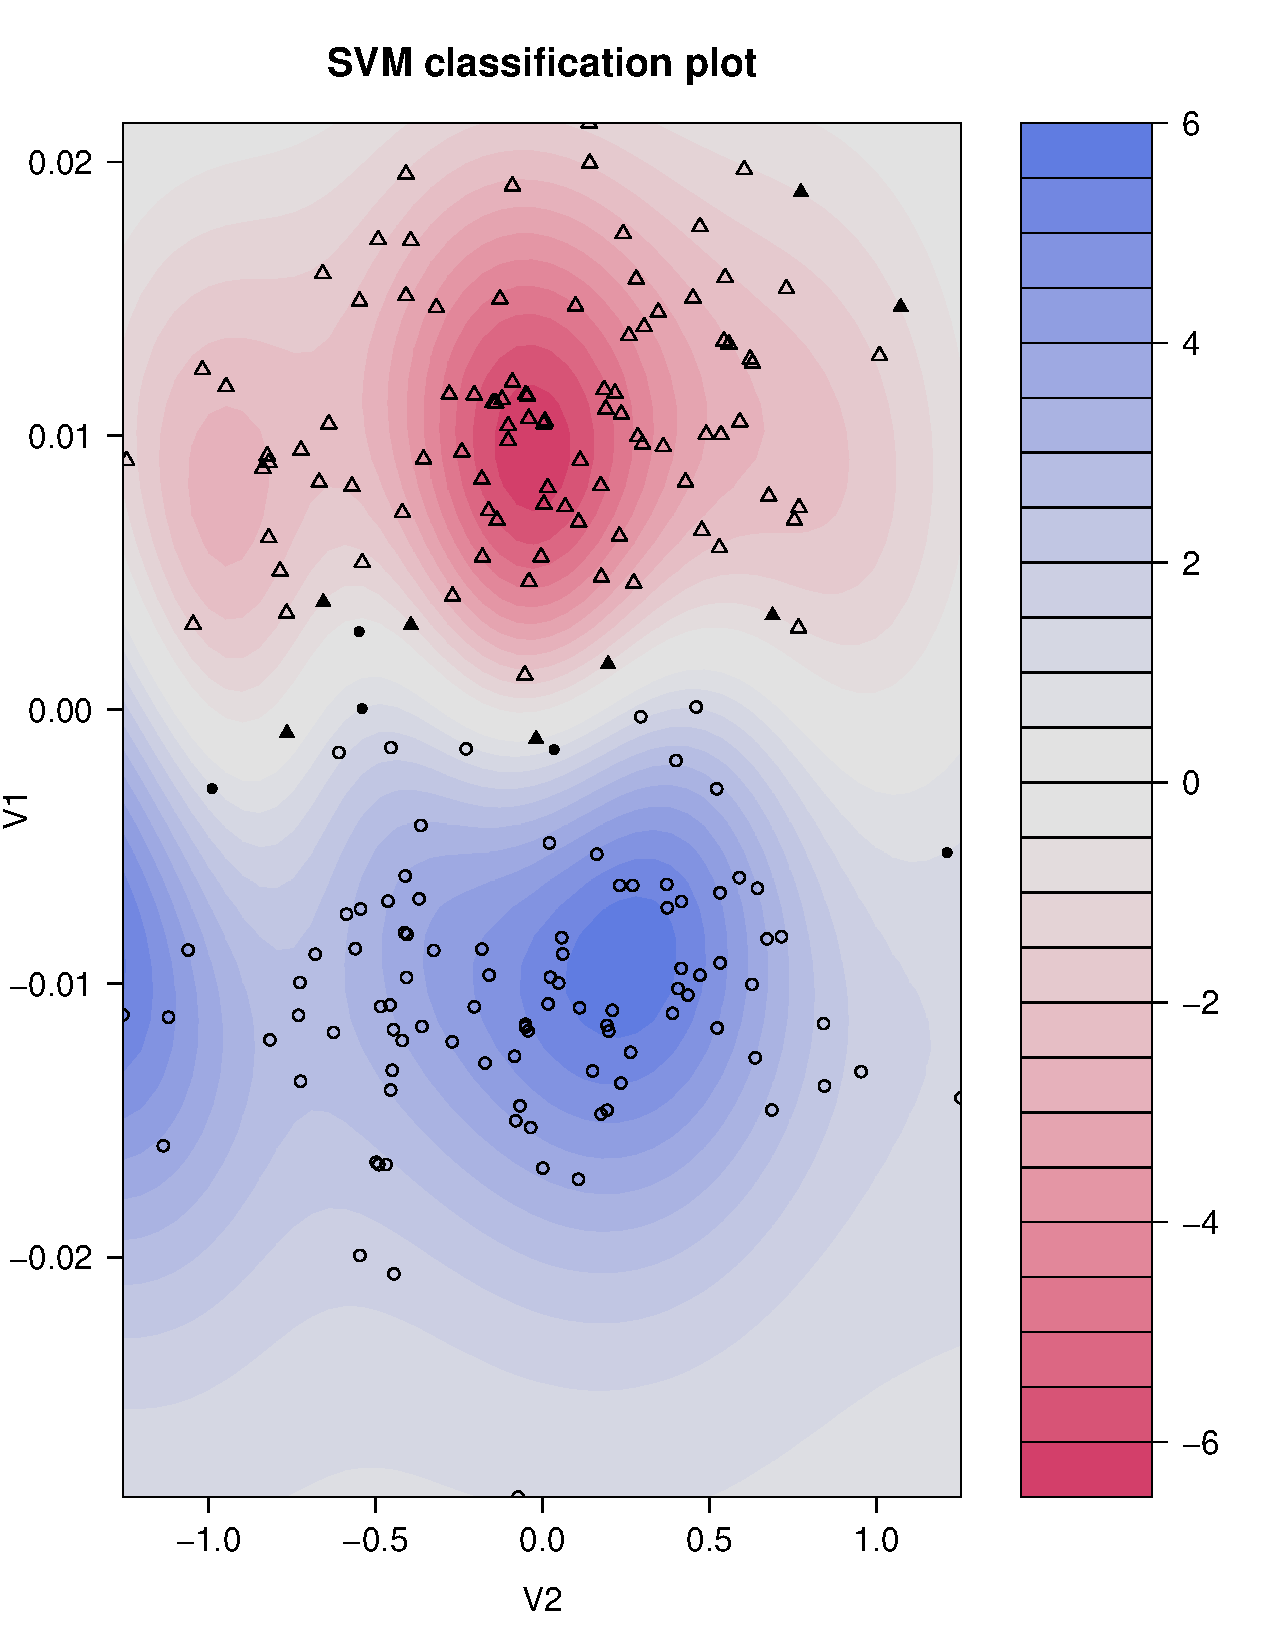
\includegraphics[width=0.5\textwidth]{bigC}
\caption{visualization with $\gamma=1$ and $C=100$ }
\label{bigC}
\end{figure}

Calculating the test error, we get errors 2\% and 3\% for C=100 and C=0.01 respectively. This is caused partly due to the fact that the test dataset is not actually a test dataset in the sense that it is a subset of the training dataset (and not new data), and partly due to the fact that the data is quite easily separable, with both hard and soft margins. 

\newpage
\subsubsection{Scaling Behavior}
We expect the number of support vector to grow more or less linearly with the number of observations and that is what we empirically observe, as shown in figure \ref{SVectors}
\begin{figure}[h!]
  \centering
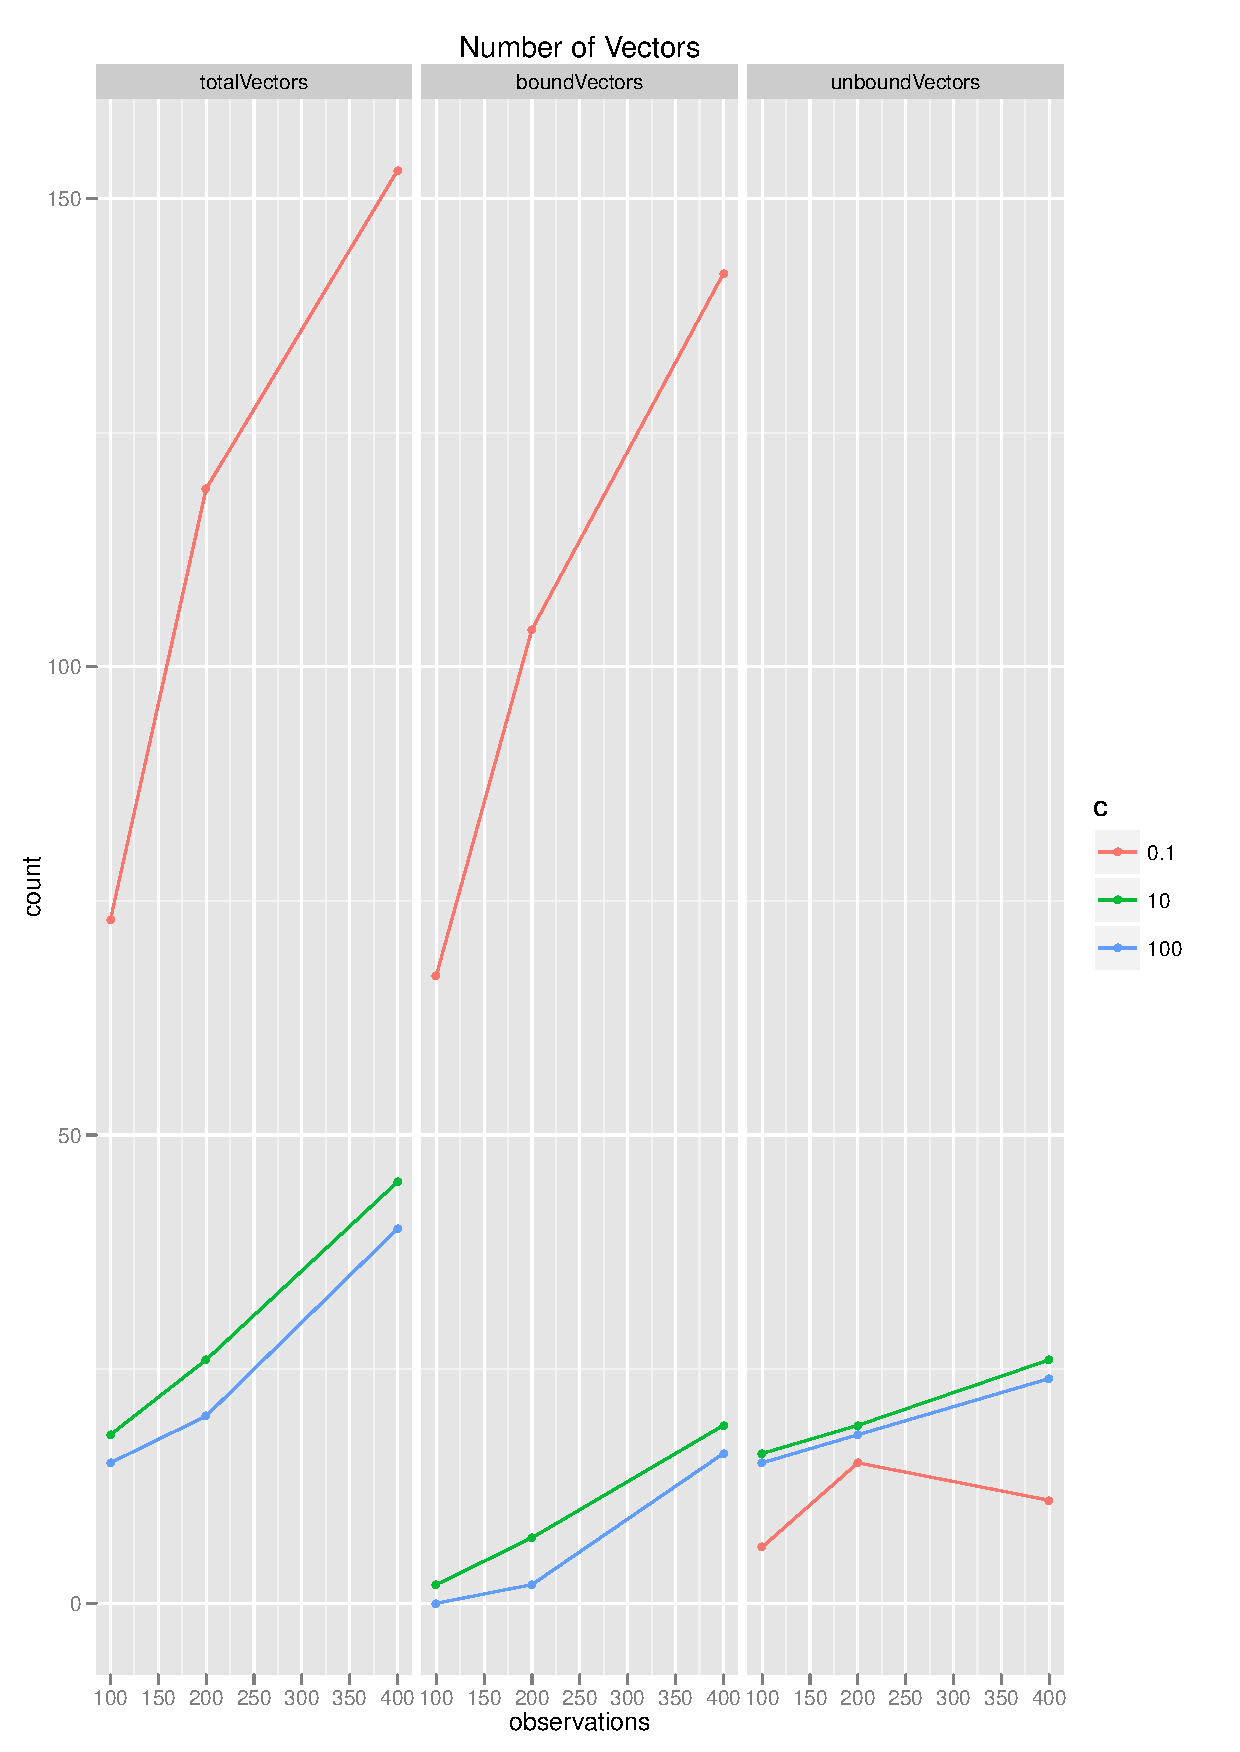
\includegraphics[width=0.5\textwidth]{SVectors}
\caption{bound, unbound, and total vectors, at different observations and different values of C}
\label{SVectors}
\end{figure}
\end{document}